\section{Zadanie 2}
\subsection{Metoda I}
Celem zadania jest wyznaczenie powyższej reprezentacji modelu dyskretnego w przestrzeni stanu. To można obliczyć za pomocą \mintinline{matlab}{tf2ss}.
\begin{minted}{matlab}
[Ad,Bd,Cd,Dd] = tf2ss(liczdys,miandys);
\end{minted}
Wynikiem są:
\begin{minted}{matlab}
Ad =

    3.2279   -1.4493    0.1738
    1.0000         0         0
         0    1.0000         0
         
Bd =

     1
     0
     0

Cd =

    0.2607   -0.2892    0.0761
    
Dd =

     0
\end{minted}
Co się przekłada na równania stanu:
\[
\left\{
\begin{array}{l}
	x_1(k)= 3,23x_1(k-1) -1,45x_2(k-1) +0,17x_3(k-1) + u(k-1) \\
	x_2(k)= x_1(k-1) \\
	x_3(k)= x_2(k-1) \\
	y(k)= 0,26x_1(k) -0,29x_2(k) + 0,08x_3(k) \\ 
\end{array}
\right.
\]
\begin{figure}[H]
\centering
 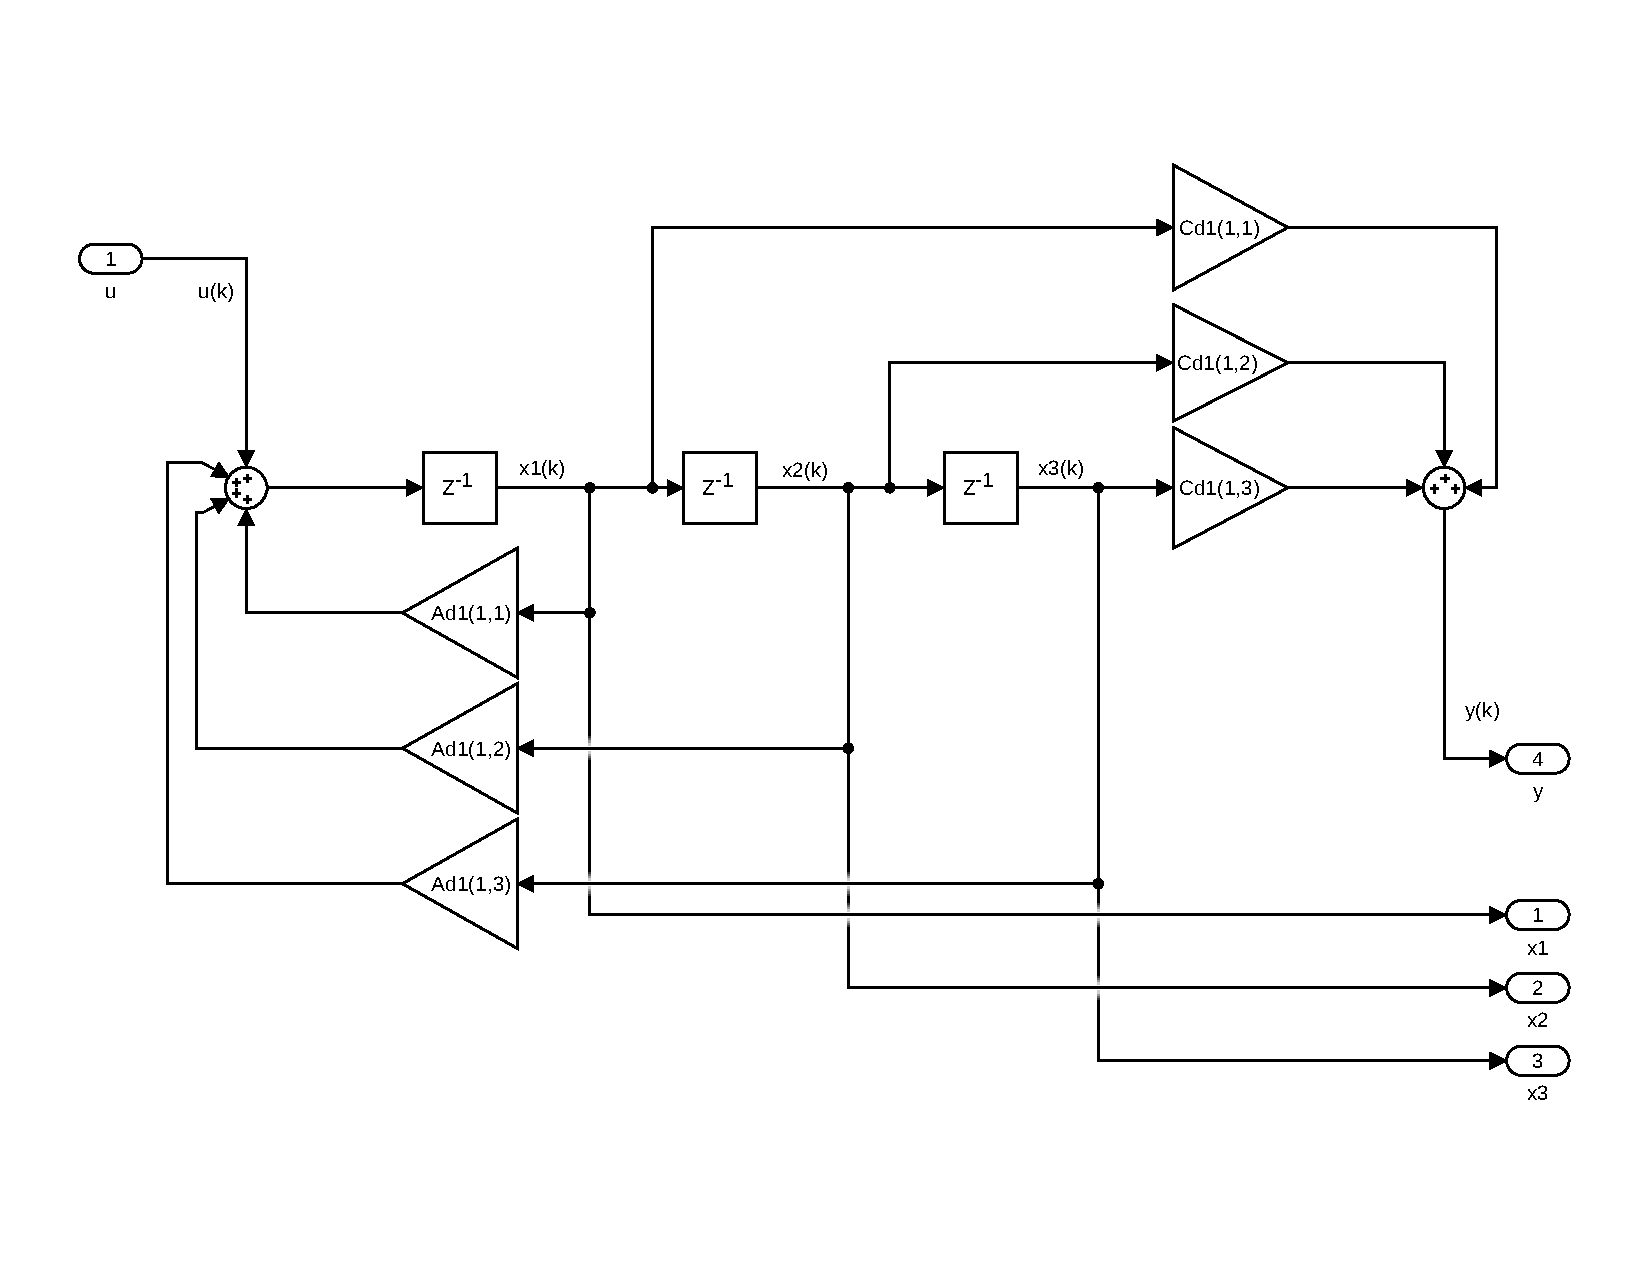
\includegraphics[width=\textwidth]{img/obj1.pdf}
\caption{Struktura modelu uzyskanego metodą I.}
\end{figure} 

\subsection{Metoda II}
Druga metoda polega na transponowaniu i zamianie wyliczonych macierzy:
\begin{minted}{matlab}
Ad2 = Ad';
Bd2 = Cd';
Cd2 = Bd';
Dd2 = Dd;
\end{minted}
Co daje nam rozwiązanie:
\begin{minted}{matlab}
Ad2 =

    3.2279    1.0000         0
   -1.4493         0    1.0000
    0.1738         0         0


Bd2 =

    0.2607
   -0.2892
    0.0761


Cd2 =

     1     0     0


Dd2 =

     0
\end{minted}
I układ równań stanu:
\[
\left\{
\begin{array}{l}
	x_1(k)= 3,23x_1(k-1) + x_2(k-1) + 0,26u(k-1) \\
	x_2(k)= -1,45x_1(k-1) + x_3(k-1) -0,29u(k-1) \\
	x_3(k)= 0,17x_1(k-1) + 0,08u(k-1) \\
	y(k)= x_1(k) \\ 
\end{array}
\right.
\]
\begin{figure}[H]
\centering
 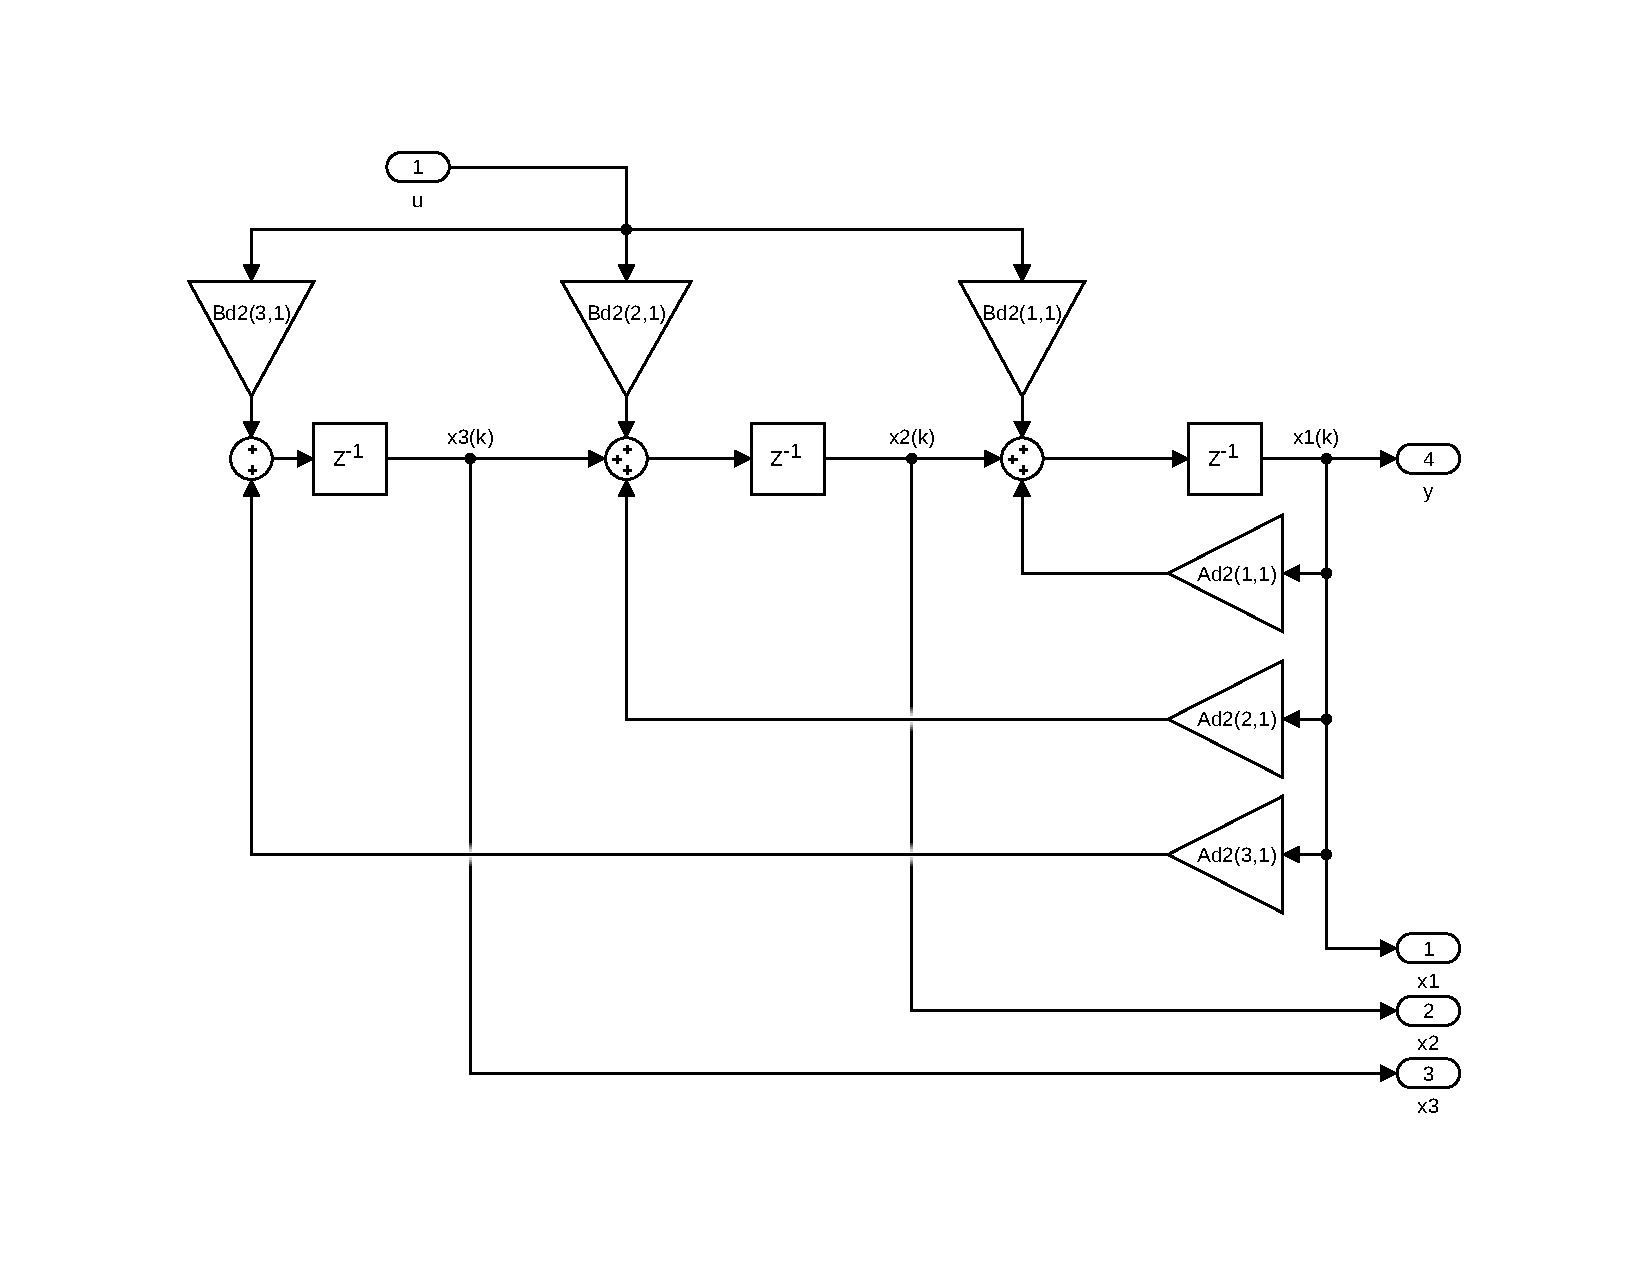
\includegraphics[width=\textwidth]{img/obj2.pdf}
\caption{Struktura modelu uzyskanego metodą II.}
\end{figure}



